\documentclass[a4paper,10pt]{article} % Uses article class in A4 format

%----------------------------------------------------------------------------------------
%	FORMATTING
%----------------------------------------------------------------------------------------

\setlength{\parskip}{0pt}
\setlength{\parindent}{0pt}
\setlength{\voffset}{-15pt}

%----------------------------------------------------------------------------------------
%	PACKAGES AND OTHER DOCUMENT CONFIGURATIONS
%----------------------------------------------------------------------------------------

\usepackage[a4paper, margin=2.5cm]{geometry} % Sets margin to 2.5cm for A4 Paper
\usepackage[onehalfspacing]{setspace} % Sets Spacing to 1.5

\usepackage[T1]{fontenc} % Use European encoding
% \usepackage[utf8]{inputenc} % Use UTF-8 encoding
\usepackage{charter} % Use the Charter font
\usepackage{microtype} % Slightly tweak font spacing for aesthetics

\usepackage[english]{babel} % Language hyphenation and typographical rules

\usepackage{amsthm, amsmath, amssymb} % Mathematical typesetting
\usepackage{marvosym, wasysym} % More symbols
\usepackage{float} % Improved interface for floating objects
\usepackage[final, colorlinks = true,
            linkcolor = black,
            citecolor = black,
            urlcolor = black]{hyperref} % For hyperlinks in the PDF
\usepackage{graphicx, multicol} % Enhanced support for graphics
\usepackage{xcolor} % Driver-independent color extensions
\usepackage{rotating} % Rotation tools
\usepackage{listings, style/lstlisting} % Environment for non-formatted code, !uses style file!
\usepackage{pseudocode} % Environment for specifying algorithms in a natural way
% \usepackage{style/avm} % Environment for f-structures, !uses style file!
\usepackage{booktabs} % Enhances quality of tables

\usepackage{tikz-qtree} % Easy tree drawing tool
\tikzset{every tree node/.style={align=center,anchor=north},
         level distance=2cm} % Configuration for q-trees
\usepackage{style/btree} % Configuration for b-trees and b+-trees, !uses style file!

\usepackage{titlesec} % Allows customization of titles
\renewcommand{\thesection}{\arabic{section}.} % Arabic numerals for the sections
\titleformat{\section}{\large}{\thesection}{1em}{}
\renewcommand{\thesubsection}{\alph{subsection})} % Alphabetic numerals for subsections
\titleformat{\subsection}{\large}{\thesubsection}{1em}{}
\renewcommand{\thesubsubsection}{\roman{subsubsection}.} % Roman numbering for subsubsections
\titleformat{\subsubsection}{\large}{\thesubsubsection}{1em}{}

\usepackage[all]{nowidow} % Removes widows

% \usepackage{csquotes} % Context sensitive quotation facilities

\usepackage[ddmmyyyy]{datetime} % Uses YEAR-MONTH-DAY format for dates
\renewcommand{\dateseparator}{.} % Sets dateseparator to '-'

\usepackage{fancyhdr} % Headers and footers
\pagestyle{fancy} % All pages have headers and footers
\fancyhead{}\renewcommand{\headrulewidth}{0pt} % Blank out the default header
\fancyfoot[L]{} % Custom footer text
\fancyfoot[C]{} % Custom footer text
\fancyfoot[R]{\thepage} % Custom footer text

\newcommand{\note}[1]{\marginpar{\scriptsize \textcolor{red}{#1}}} % Enables comments in red on margin


% argmin
\DeclareMathOperator*{\argmin}{arg\,min}

% code highlighting
\usepackage{minted}
\usepackage{fontspec}

\setmainfont{Optima}
\setmonofont{Fira Code}
\setminted{fontsize=\footnotesize}

% Custom section titles
\usepackage{titlesec}
\titleformat*{\section}{\bf \Large}
\titleformat*{\subsection}{\bf \large}
\titleformat*{\subsubsection}{\bf \normalsize}

% Fancy tables
\usepackage{tabularx}
\usepackage{multirow}

% Grid of images
\usepackage{subfig}

%----------------------------------------------------------------------------------------

\begin{document}

%----------------------------------------------------------------------------------------
%	TITLE SECTION
%----------------------------------------------------------------------------------------

\title{template_assignment} % Article title
\fancyhead[C]{}

\begin{minipage}{0.295\textwidth} % Left side of title section
\raggedright
Mobile Robotics\\ % Your lecture or course
\footnotesize % Authors text size
%\hfill\\ % Uncomment if right minipage has more lines
\href{https://sayan.page}{Sayan Goswami} % Your name, your matriculation number
\medskip % \hrule
\end{minipage}
\begin{minipage}{0.4\textwidth} % Center of title section
\centering
\large % Title text size
Final Project Report\\ % Assignment title and number
% \normalsize % Subtitle text size
% Subtitle\\ % Assignment subtitle
\end{minipage}
\begin{minipage}{0.295\textwidth} % Right side of title section
\raggedleft
\today\\ % Date
\footnotesize % Email text size
% \hfill\\ % Uncomment if left minipage has more lines
\href{mailto:email@sayan.page}{email@sayan.page}% Your email
\medskip % \hrule
\end{minipage}
\hrule

%----------------------------------------------------------------------------------------
%	ARTICLE CONTENTS
%----------------------------------------------------------------------------------------

\section{Localization}

This part of the project involves the implementation of the Markov localization algorithm and  successfully performing localization in a given environment with no information regarding the initial position of the robot in the environment.

\subsection{Environment}

The environment used is a grid world with walls surrounding the edges as well as walls within the grid.
This is chosen because it can be extended with minimal effort to work with occupancy grid based map representations.

The landmarks that the localization algorithms uses is the state (free or walled) of the neighbouring cells in the lateral and vertical directions.
Using these landmarks, the algorithm can form an estimate of the possible locations in the map where the robot is possibly located at.
This is done during the perception stage of localization.

\subsection{Robot \& Sensing}

The robot has limited sensing capabilities.
It is able to detect whether it's first degree neighbors in the lateral and vertical direction are free cells or if they are walled cells.
This can be thought of as primitive rangefinder.
The sensor is accurate with it's readings with a probability of unity and there are multiple poses on the map where the robot can obtain the same sensor readings.
This is handled by the localization algorithm during the perception stage.
The posterior probabilities are normalized so that they sum to unity.

\subsection{Movement \& Motion Model}

The robot is able to move in four directions —- up, down, left and right on the map.
The movement in a chosen direction succeeds with a probability of unity if the cell it wants to move to is free.
If the cell is walled, the robot stays at its previous location.
Thus, if the robot is at pose $(row_i, col_j)$ at time $t$, then it can be either at $(row_i, col_j)$ or either of the four neighbouring cells ($(row_{i - 1}, col_{j})$, $(row_{i + 1}, col_{j})$, $(row_{i}, col_{j - 1})$, $(row_{i}, col_{j + 1})$) based on the intended direction of movement at time $t + 1$.

\subsection{Localization Module}

The localization module \footnote{The code for the localization module is available at \href{https://github.com/say4n/mobile-robotics}{https://github.com/say4n/mobile-robotics}.} is split into two subparts corresponding to the perception and the prediction stages of the localization algorithm.
The algorithm used for localization is the Markov localization algorithm.
The robot executes a set of actions in the environment.
The actions of the robot correspond to the predication stage of the localization algorithm.
The perception stages of the localization algorithm are interleaved between the actions.
The various components are described in the following pages.

\hfill
\newpage

\subsubsection*{Initial Belief}

\begin{minipage}{0.5\textwidth}
    \flushleft
    The initial belief of the localization algorithm is set to an uniform distribution over all the possible states that it can occupy.
    This is shown in figure \ref{fig:1}.
    The hatched out cells represent walls in the environment.
    The numbers on the cells represent the belief of the localization algorithm.
    The red outlined cell is the actual position of the robot, this is unknown to the localization algorithm.
    Belief initialization is performed as follows.

    \begin{minted}{python}
n_rows = env.get_n_rows()
n_cols = env.get_n_cols()
free_cells = env.get_free_cells()

belief = np.zeros((n_rows, n_cols))
for cell in free_cells:
    r, c = cell
    belief[r, c] = 1/len(free_cells)
    \end{minted}
\end{minipage} %
\hspace{0.05\textwidth} %
\begin{minipage}{0.4\textwidth}
    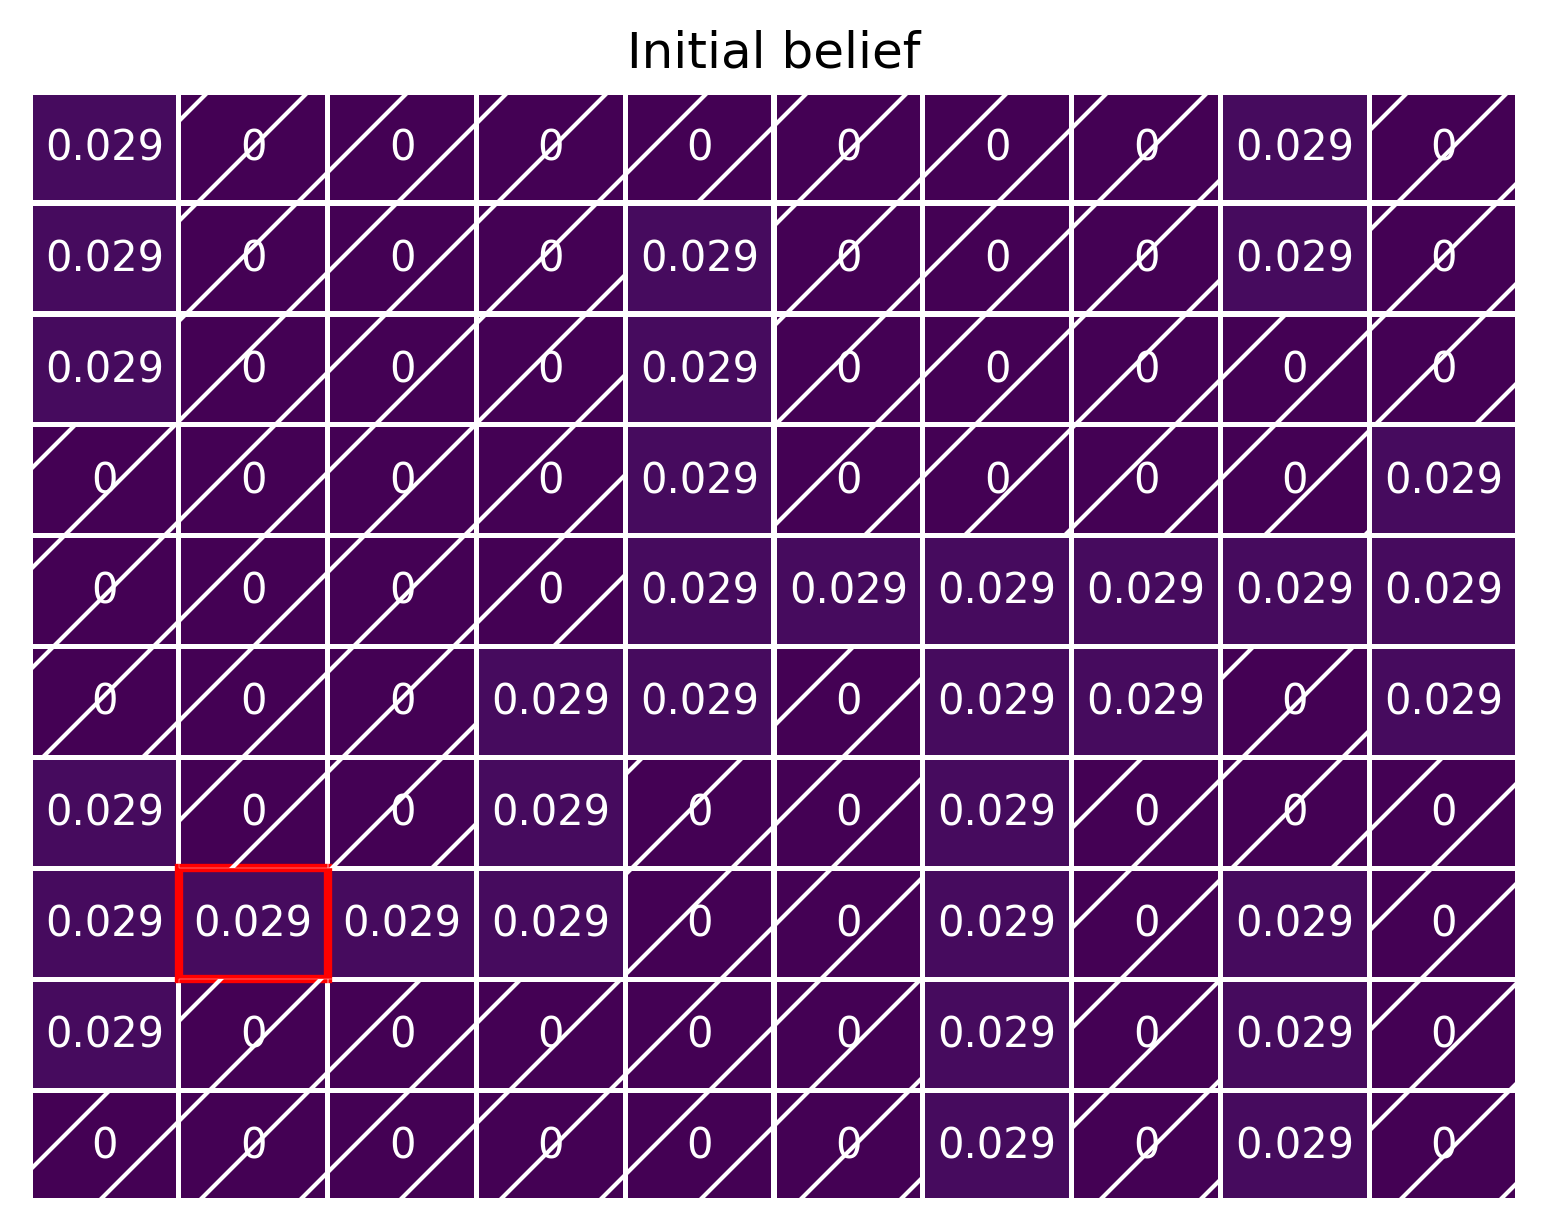
\includegraphics[width=\linewidth]{maps/Initial belief.png}
    \captionof{figure}{The localization algorithm starts with an uniform initial belief and then updates it's estimate via perception and prediction.}
    \label{fig:1}
\end{minipage}

\subsubsection*{Perception Stage}

During this phase, the robot uses its exteroceptive sensors to correct its previous estimate of its pose in the map.
The uncertainty in the pose estimate decreases during this stage.
This is implemented in the following code block.

\begin{minted}{python}
# See phase.
obs = env.sense()
possible_locs = env.get_possible_locations_given_observation(obs)

# Computer posterior probabilities.
posteriors = np.zeros(len(possible_locs))
for i, (r, c) in enumerate(possible_locs):
    # Assuming perfect sensing.
    posteriors[i] = 1 * belief[r][c]

# Normalize probabilities.
# breakpoint()
posteriors = posteriors / np.sum(posteriors)

# Update beliefs.
belief = np.zeros(belief.shape)
for i, (r, c) in enumerate(possible_locs):
    belief[r][c] = posteriors[i]
\end{minted}

\subsubsection*{Prediction Stage}

During this stage, the robot uses its proprioceptive sensors to estimate its pose.
The uncertainty in the pose estimate increases during this stage as it the robot also performs a move action.
This is implemented in the following code block.

\begin{minted}{python}
# Act phase.
direction = action[1]
env.act(direction)

# Keep a copy of previous beliefs.
belief_copy = deepcopy(belief)

# Re-initialize beliefs.
belief = np.zeros(belief.shape)

# Update beliefs.
non_zero_probability_cells = np.argwhere(belief_copy > 0)
for r, c in non_zero_probability_cells:
    next_r, next_c = env.get_next_state(direction, (r, c))
    # Assuming single possible movement here.
    # Else, needs to be divided by number of possible next states.
    belief[next_r][next_c] += belief_copy[r][c]
\end{minted}

\subsubsection*{Localization in Action}

A sample run of the localization algorithm is illustrated in figure \ref{fig:2}.
As can be observed from the figure, the localization algorithm is able to locate the robot in the grid world after just 5 steps.
After this, the robot's pose predicted by the localization algorithm perfectly matches the actual pose of the robot in the environment.

\begin{figure}[!htbp]
    \begin{tabular}{ccc}
        \subfloat[Perception.]{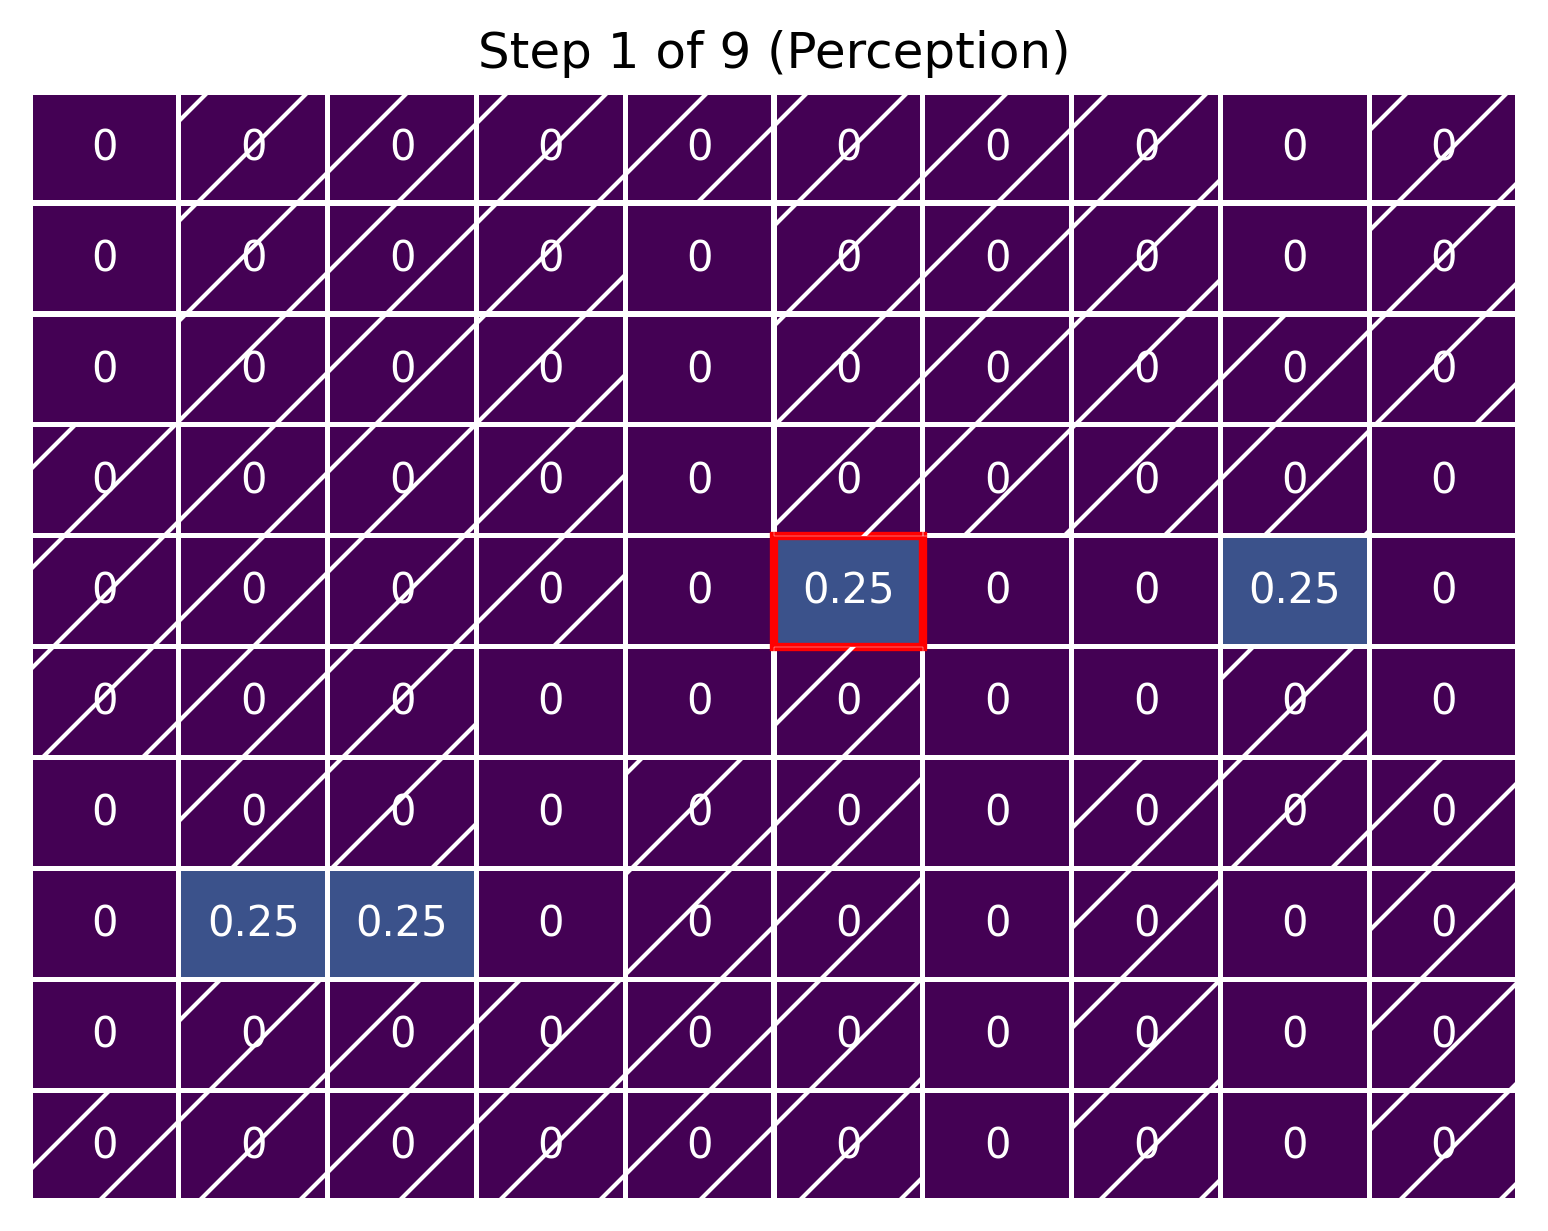
\includegraphics[width = 0.3\textwidth]{maps/Step 1 of 9 (Perception).png}} &
        \subfloat[Prediction after moving left.]{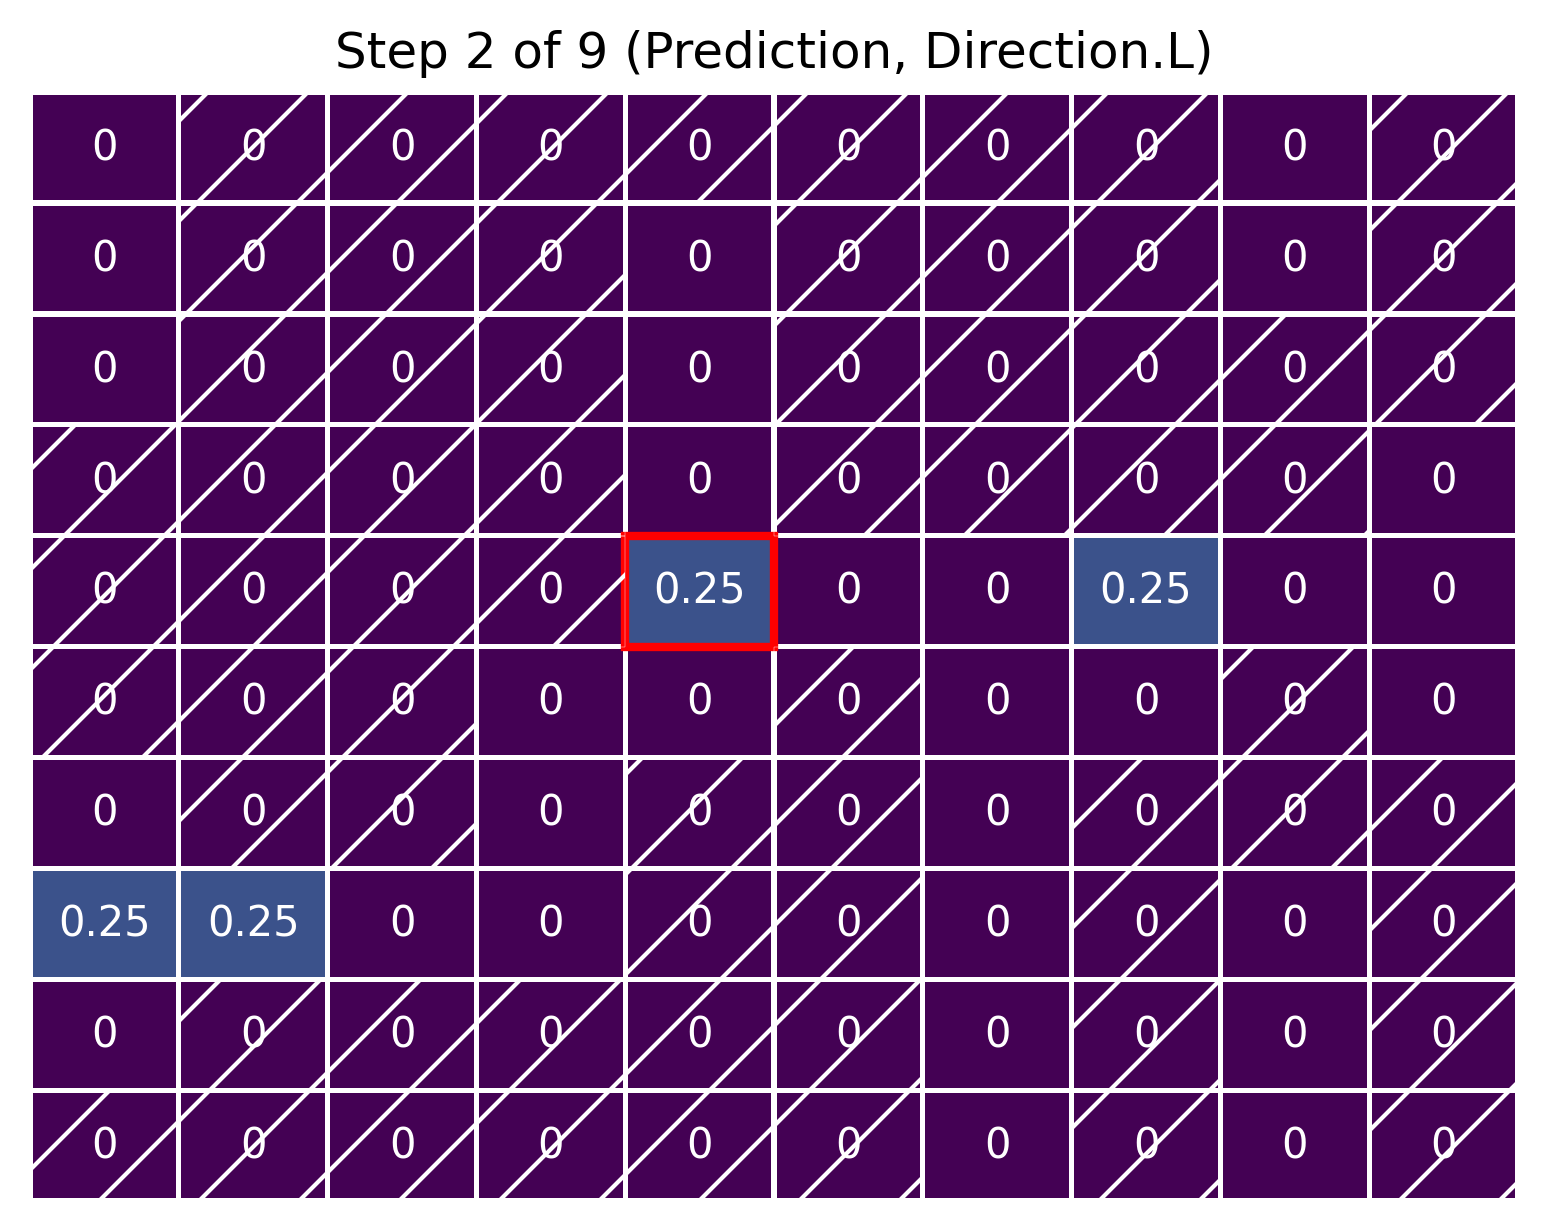
\includegraphics[width = 0.3\textwidth]{maps/Step 2 of 9 (Prediction, Direction.L).png}} &
        \subfloat[Perception.]{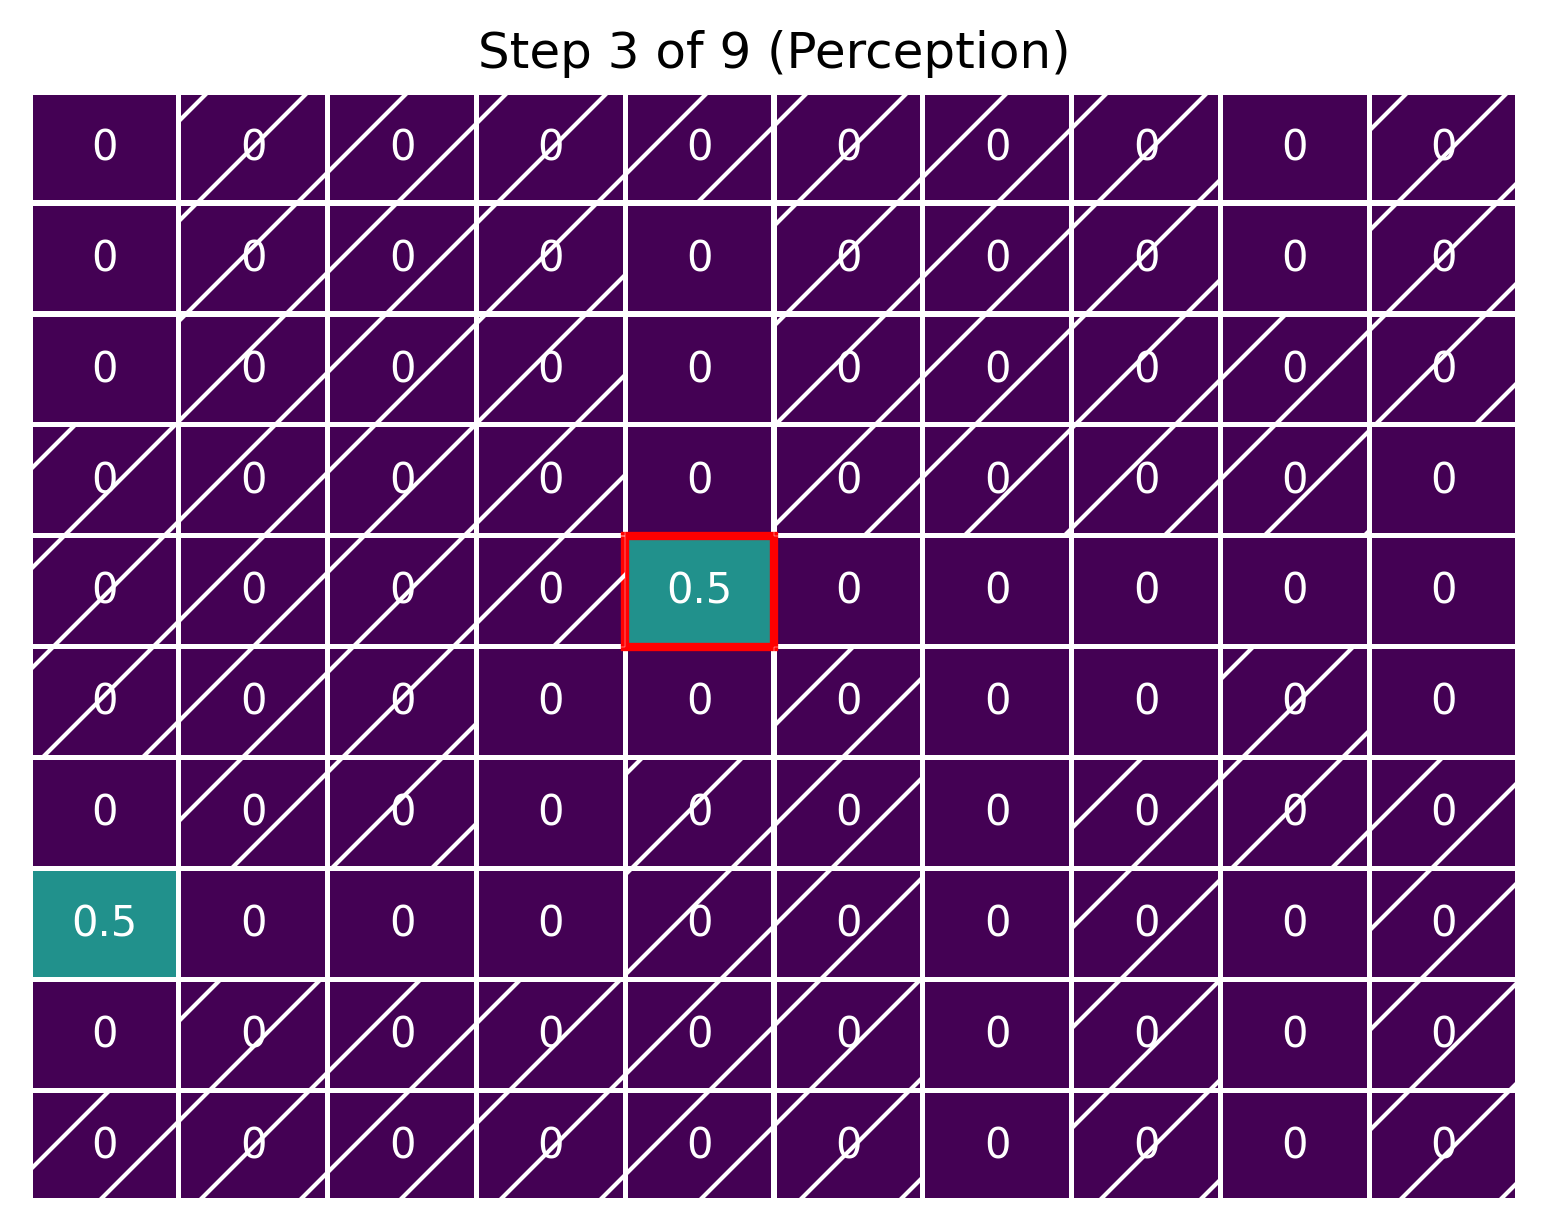
\includegraphics[width = 0.3\textwidth]{maps/Step 3 of 9 (Perception).png}} \\
        \subfloat[Prediction after moving up.]{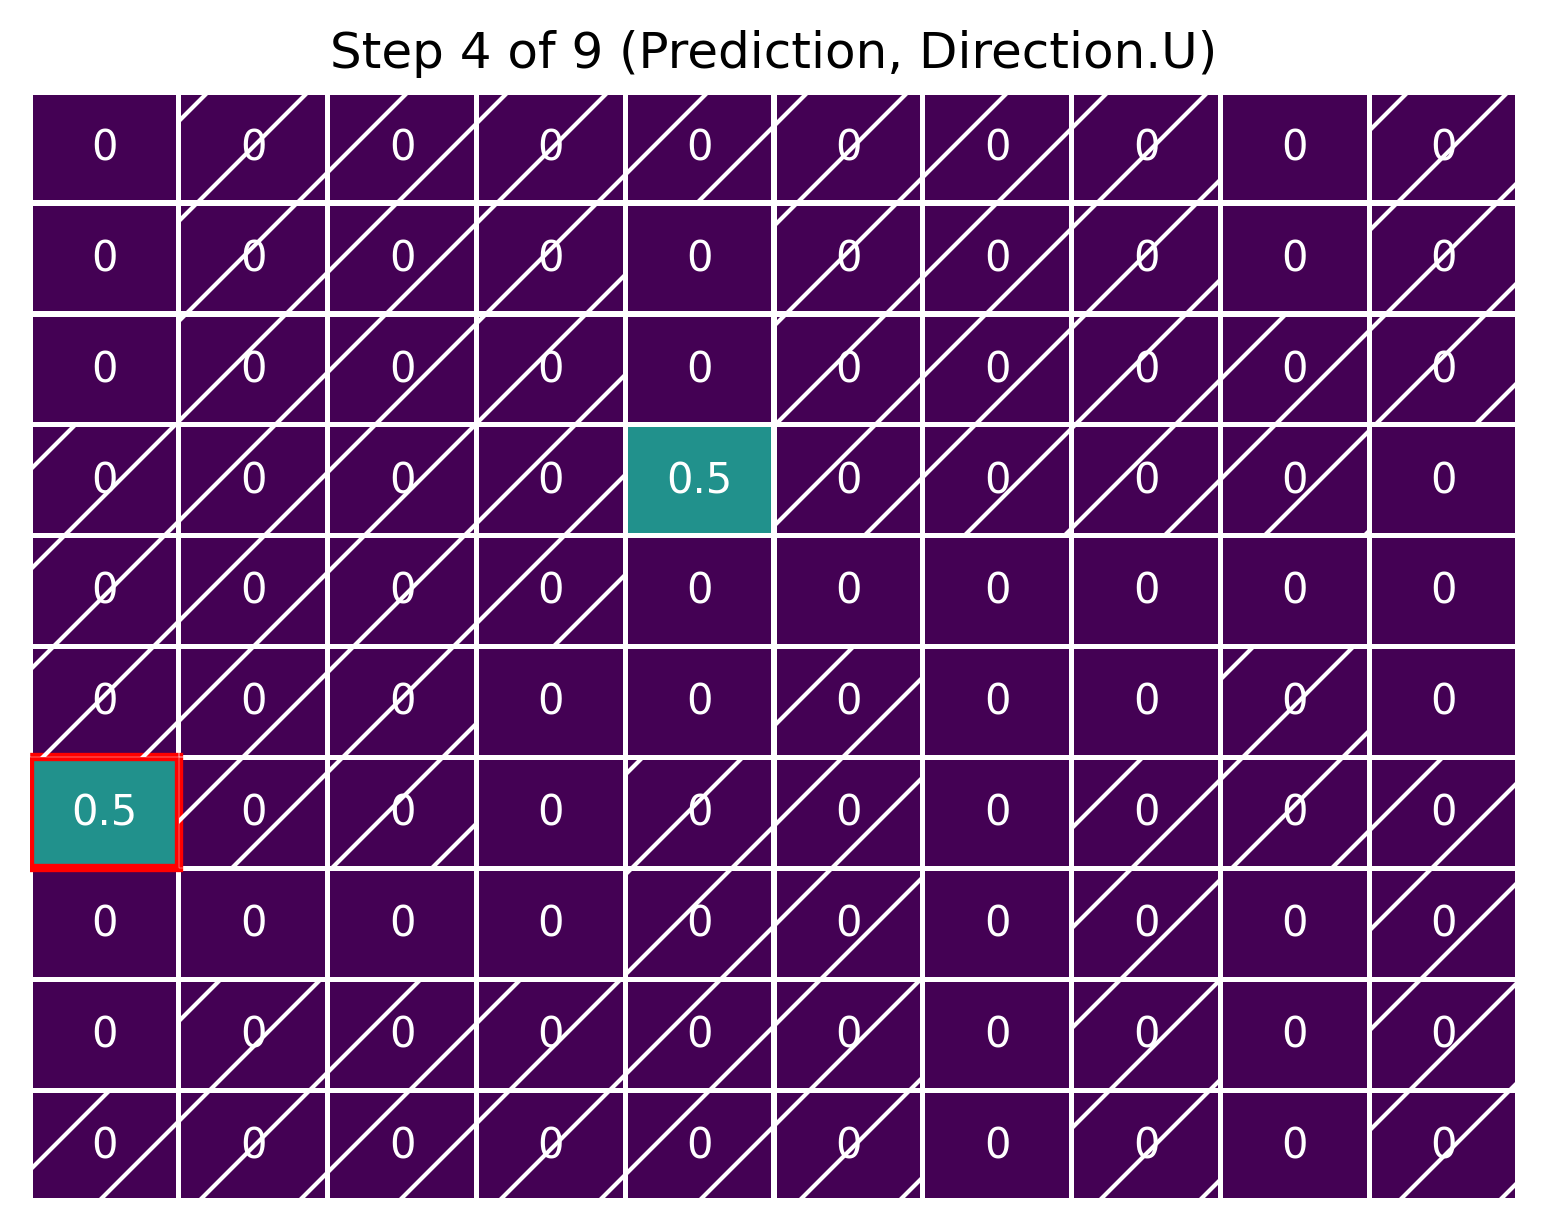
\includegraphics[width = 0.3\textwidth]{maps/Step 4 of 9 (Prediction, Direction.U).png}} &
        \subfloat[Perception.]{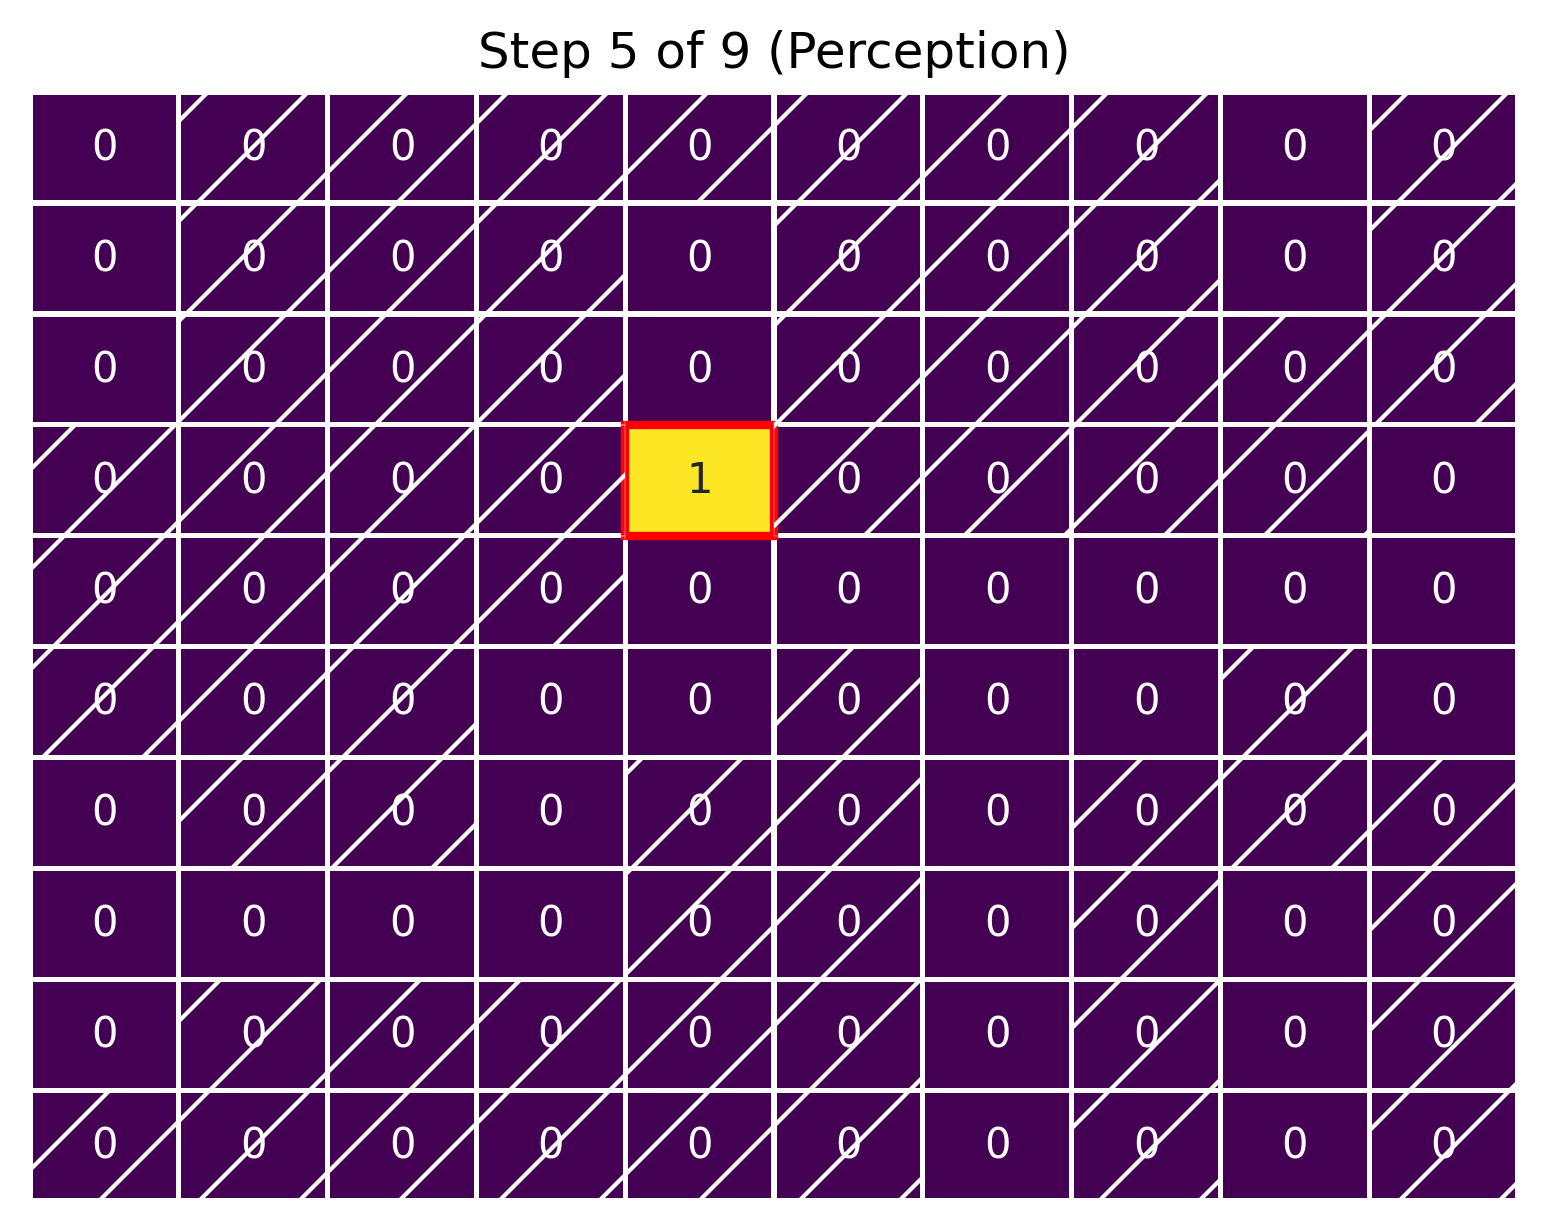
\includegraphics[width = 0.3\textwidth]{maps/Step 5 of 9 (Perception).png}} &
        \subfloat[Prediction after moving down.]{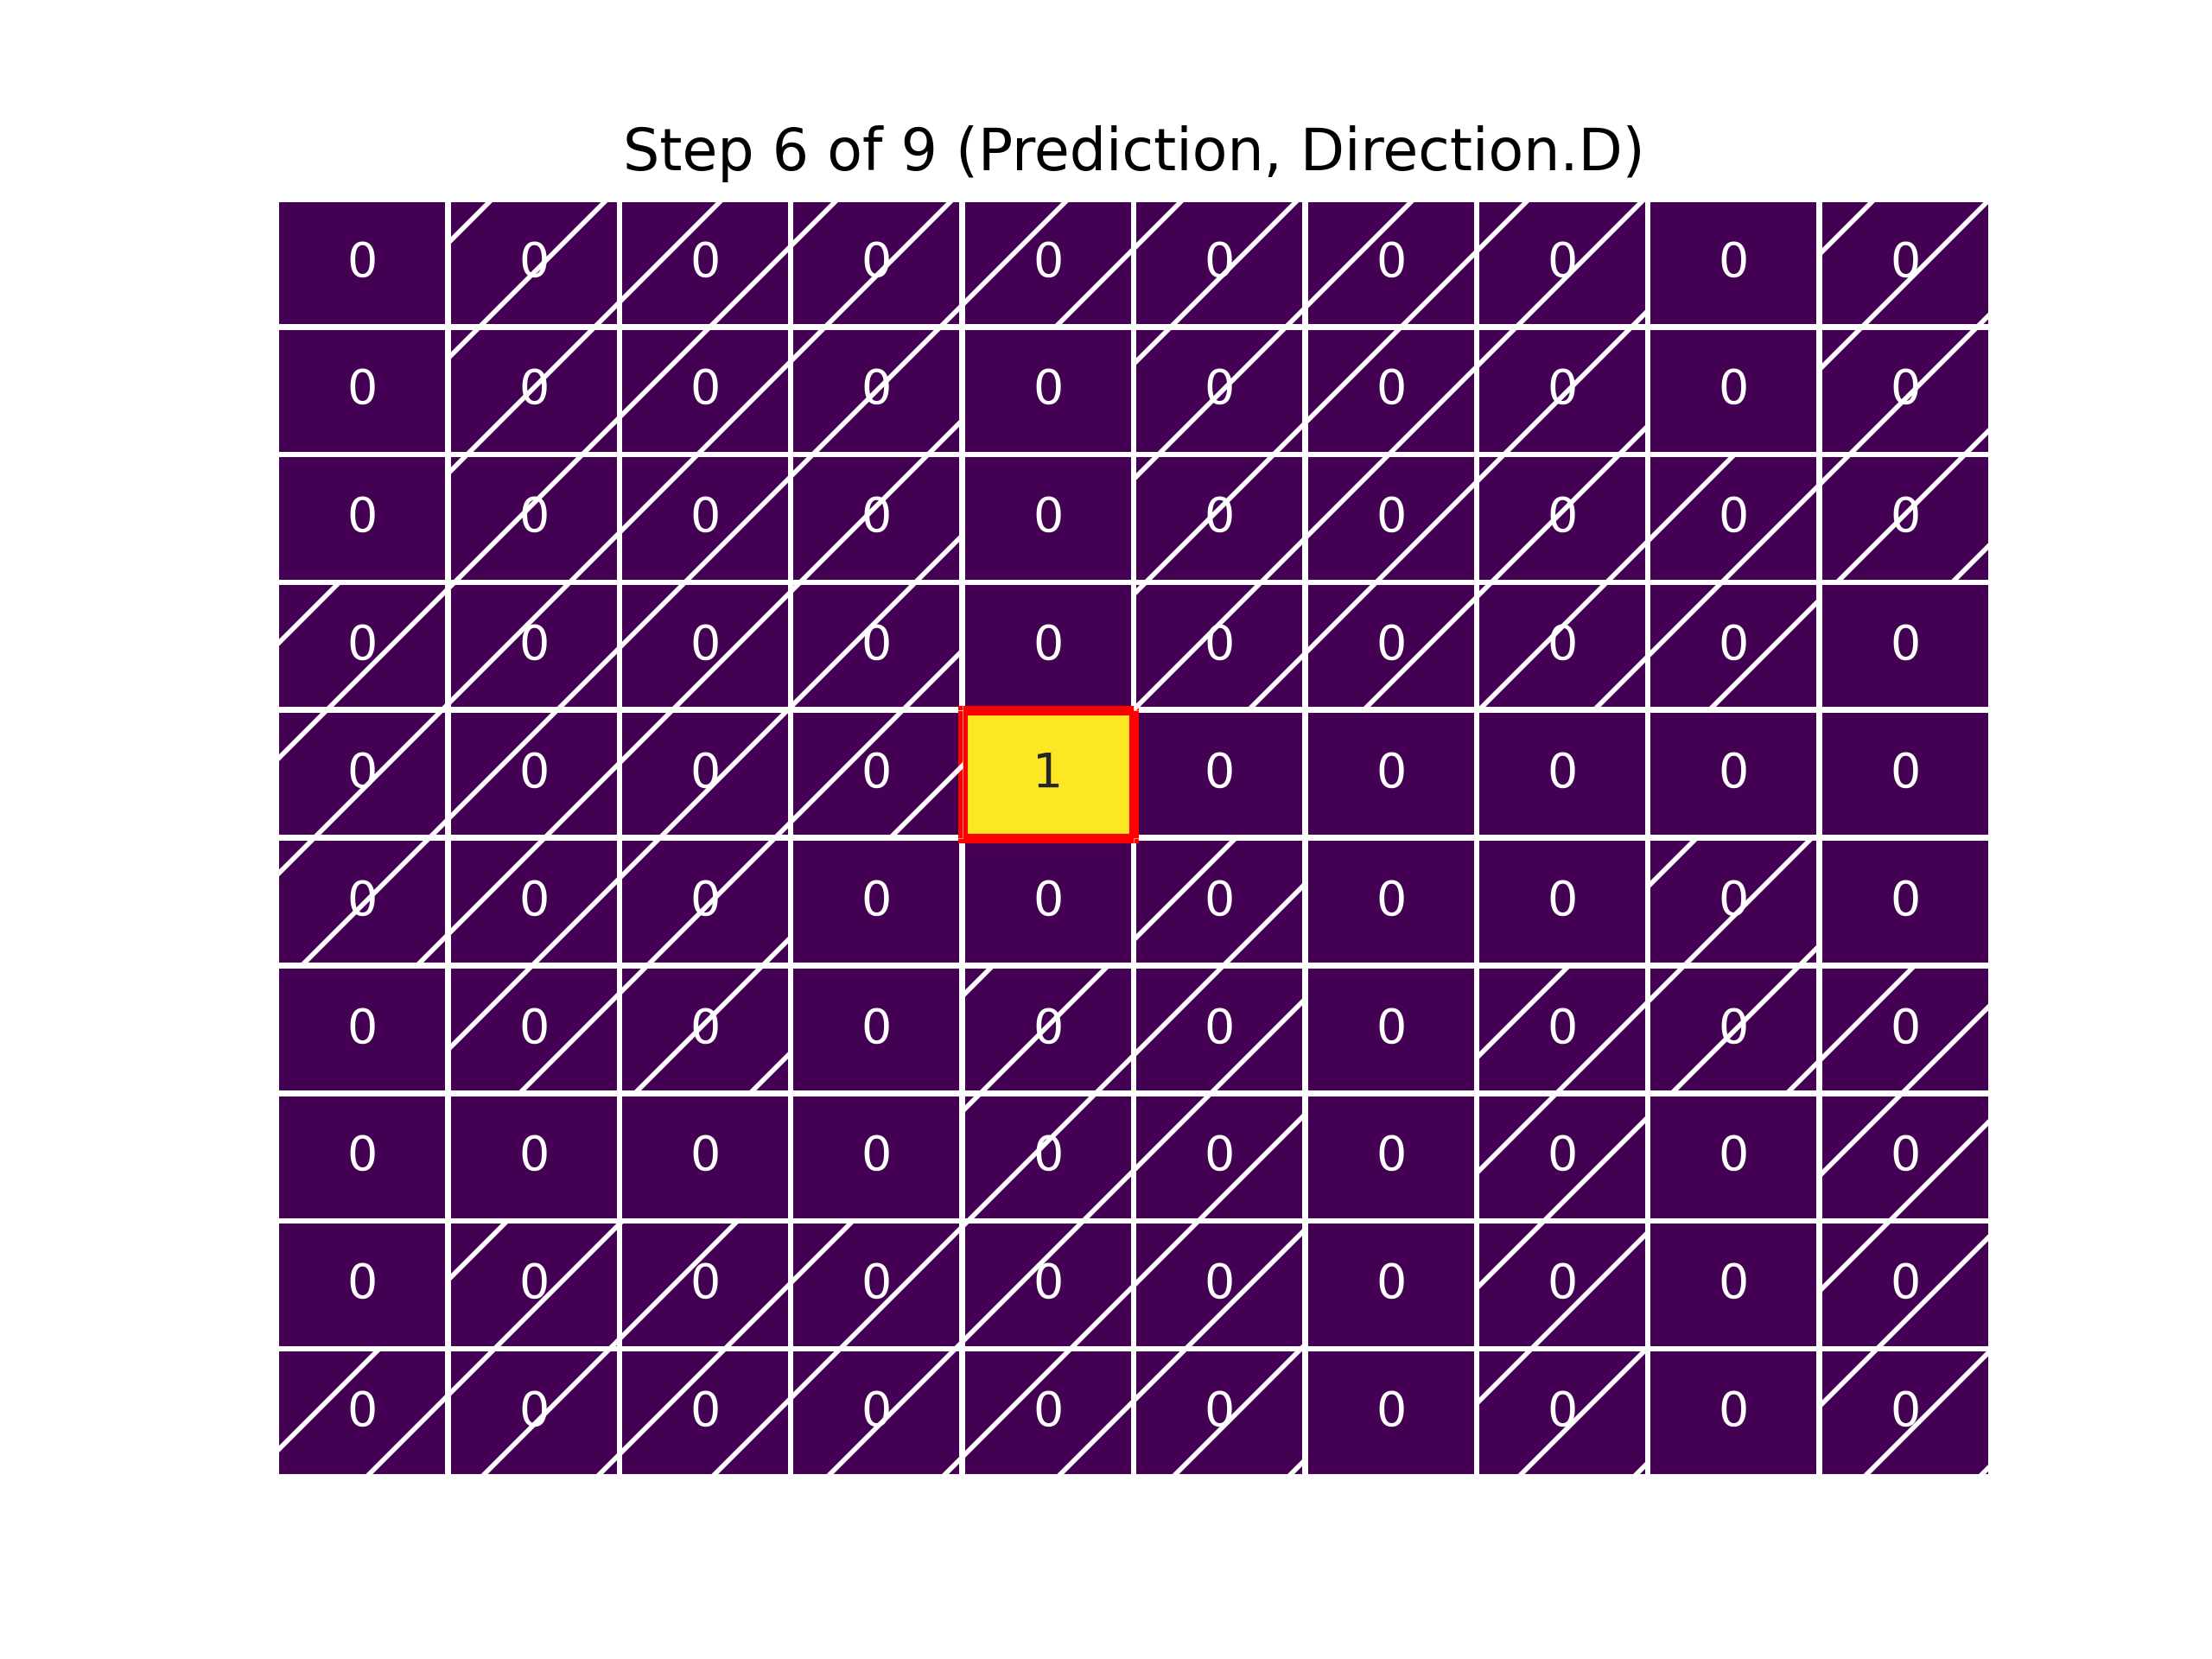
\includegraphics[width = 0.3\textwidth]{maps/Step 6 of 9 (Prediction, Direction.D).png}} \\
        \subfloat[Perception.]{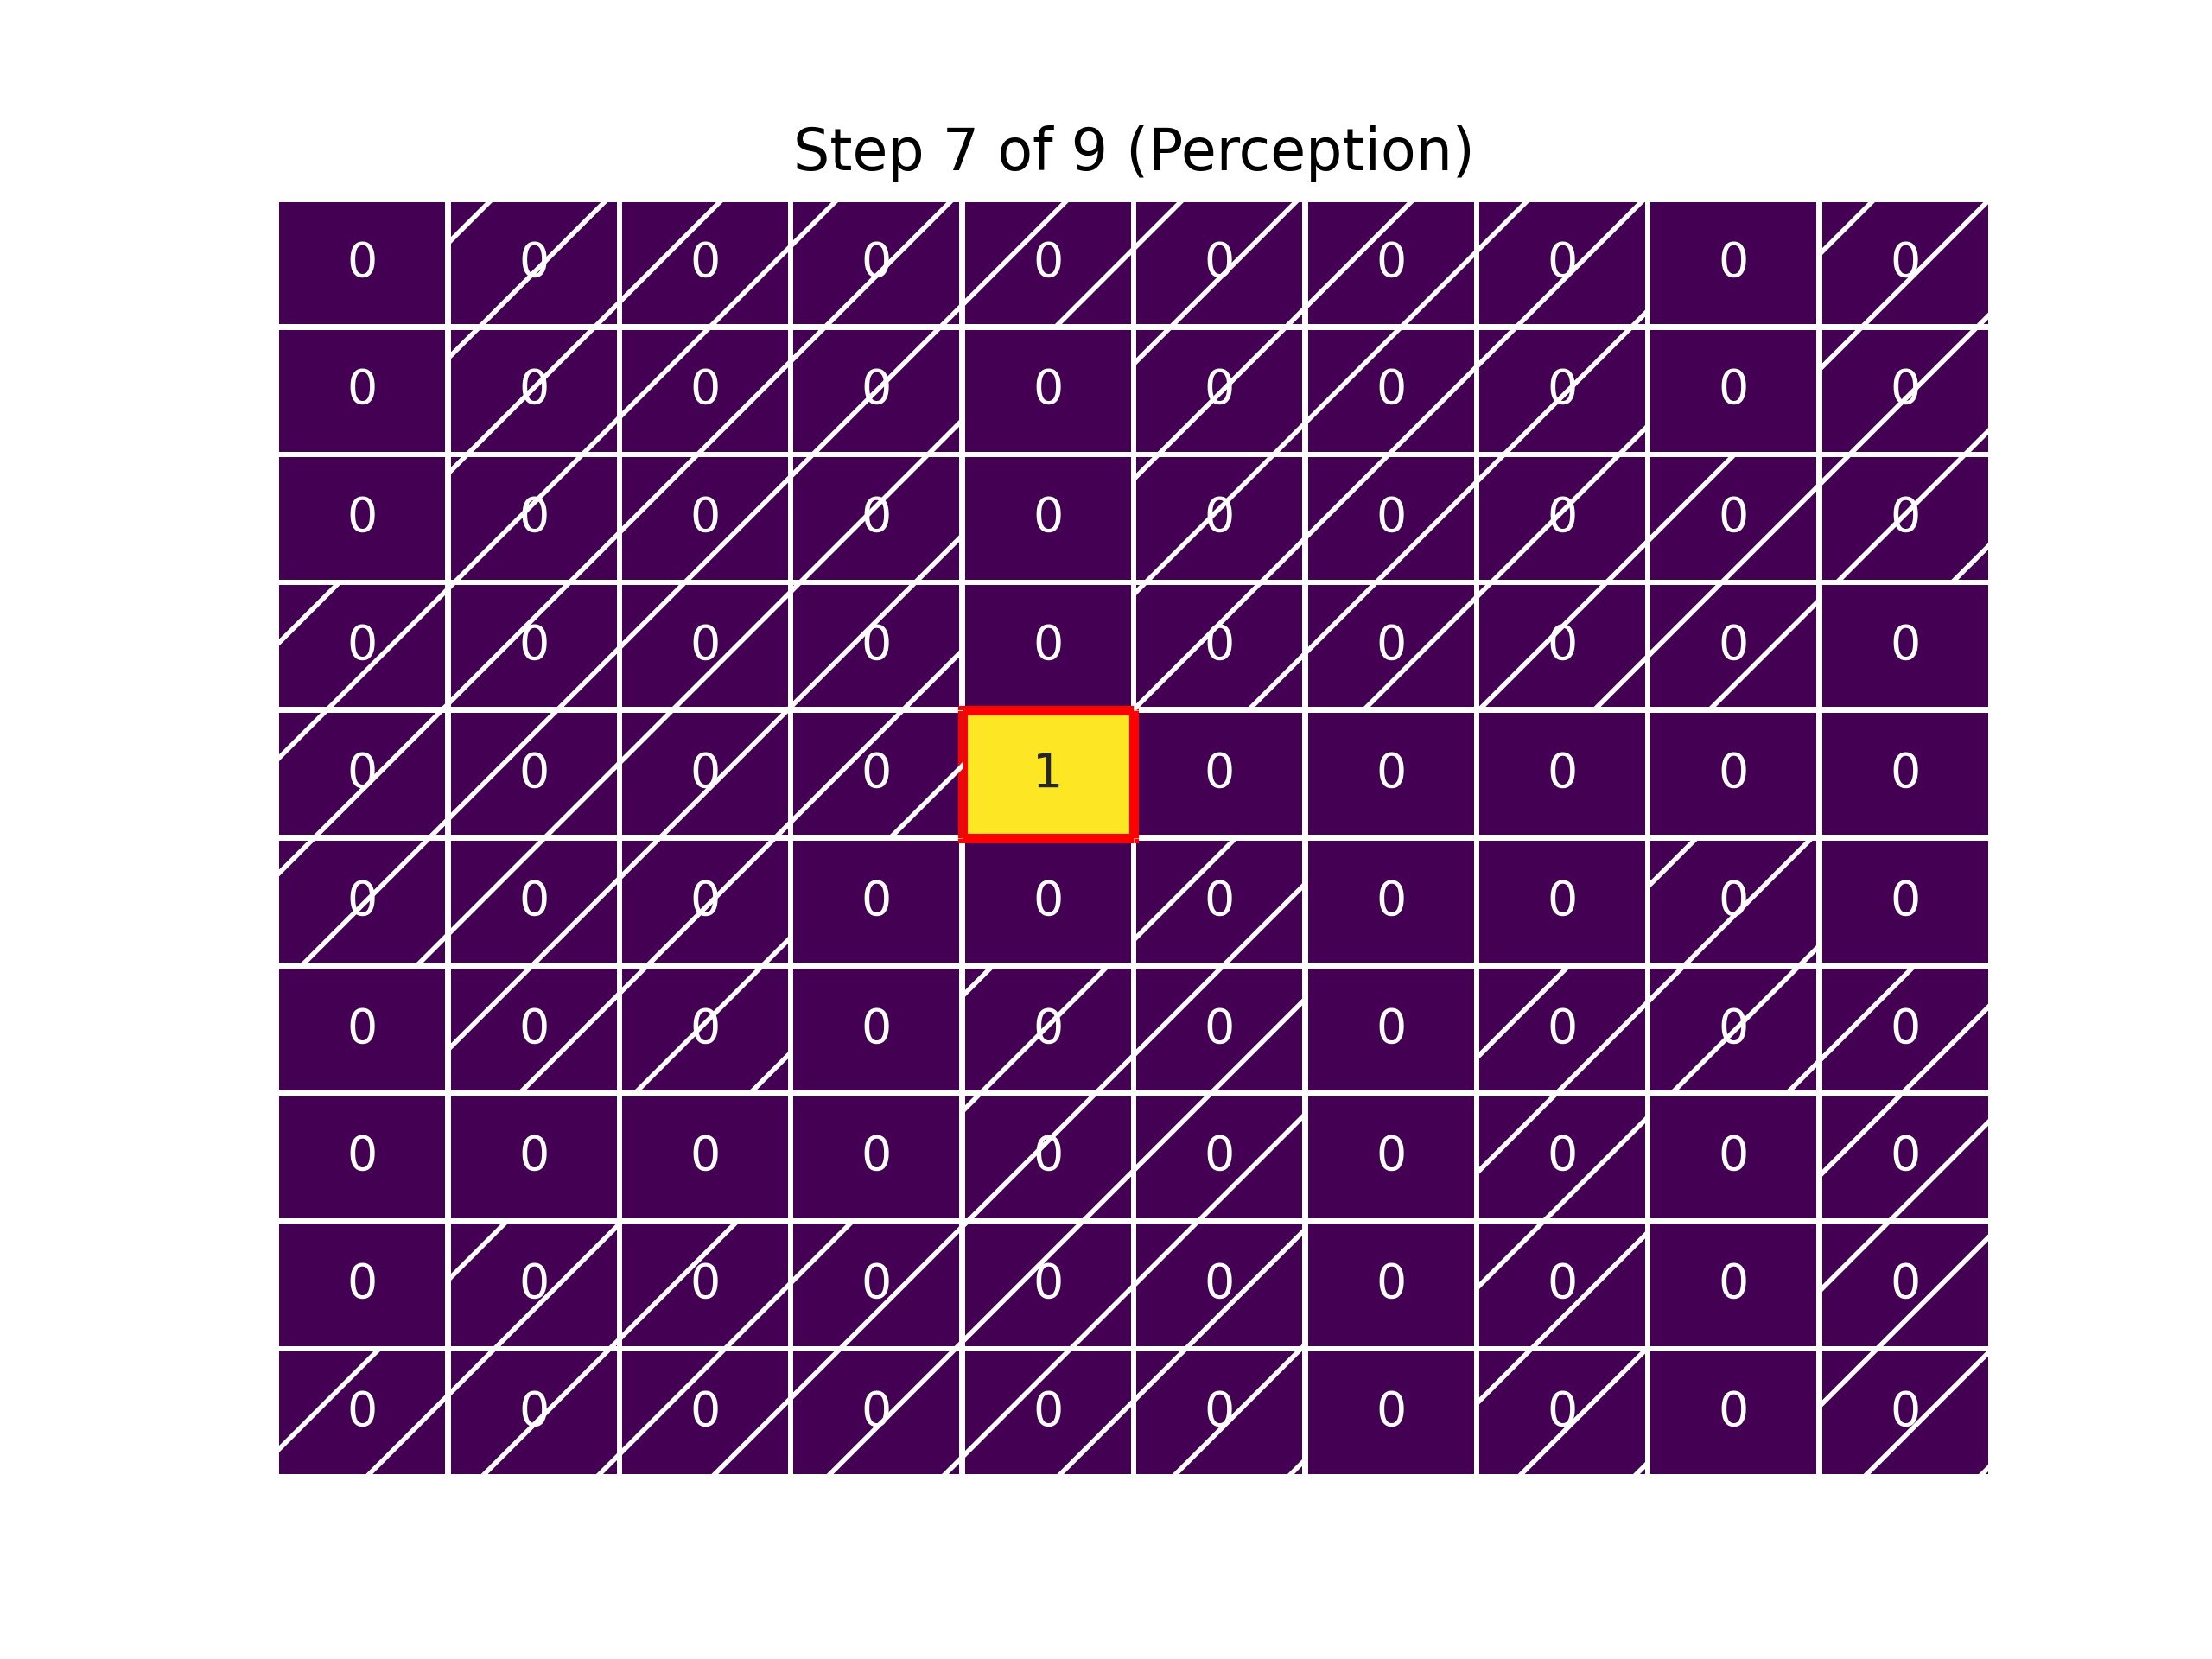
\includegraphics[width = 0.3\textwidth]{maps/Step 7 of 9 (Perception).png}} &
        \subfloat[Prediction after moving right.]{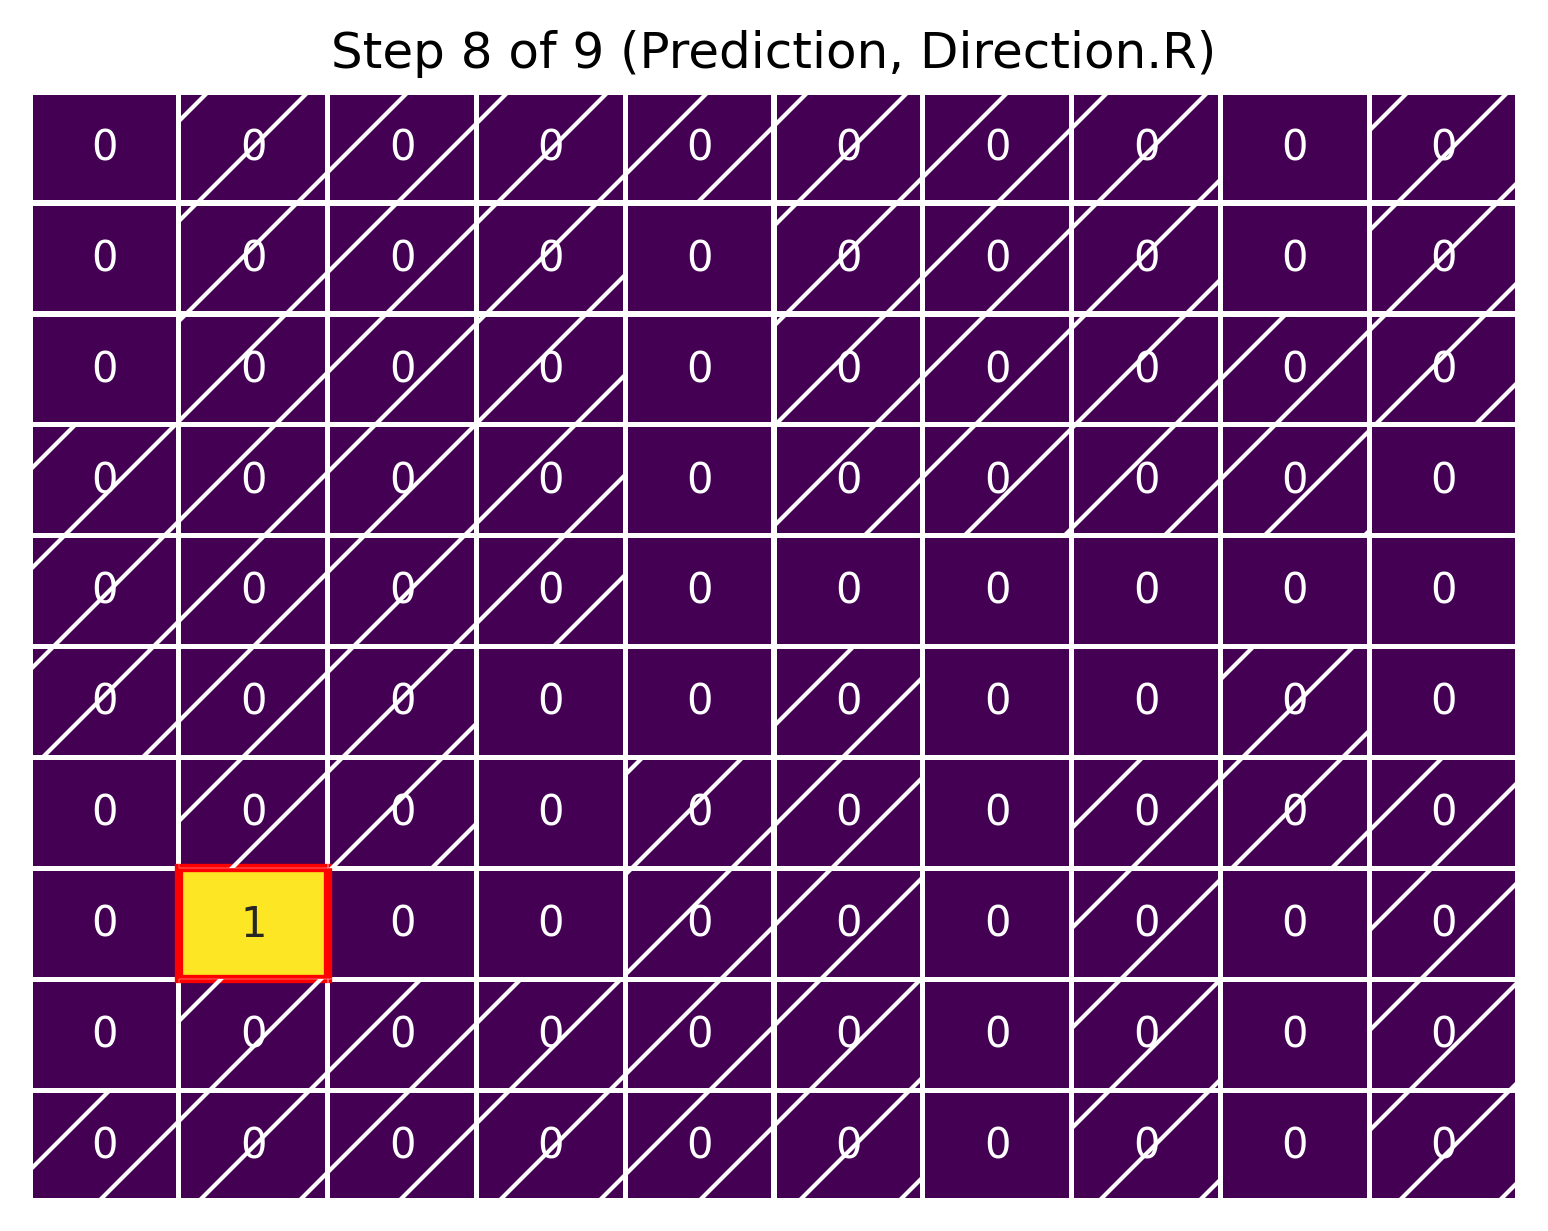
\includegraphics[width = 0.3\textwidth]{maps/Step 8 of 9 (Prediction, Direction.R).png}} &
        \subfloat[Perception.]{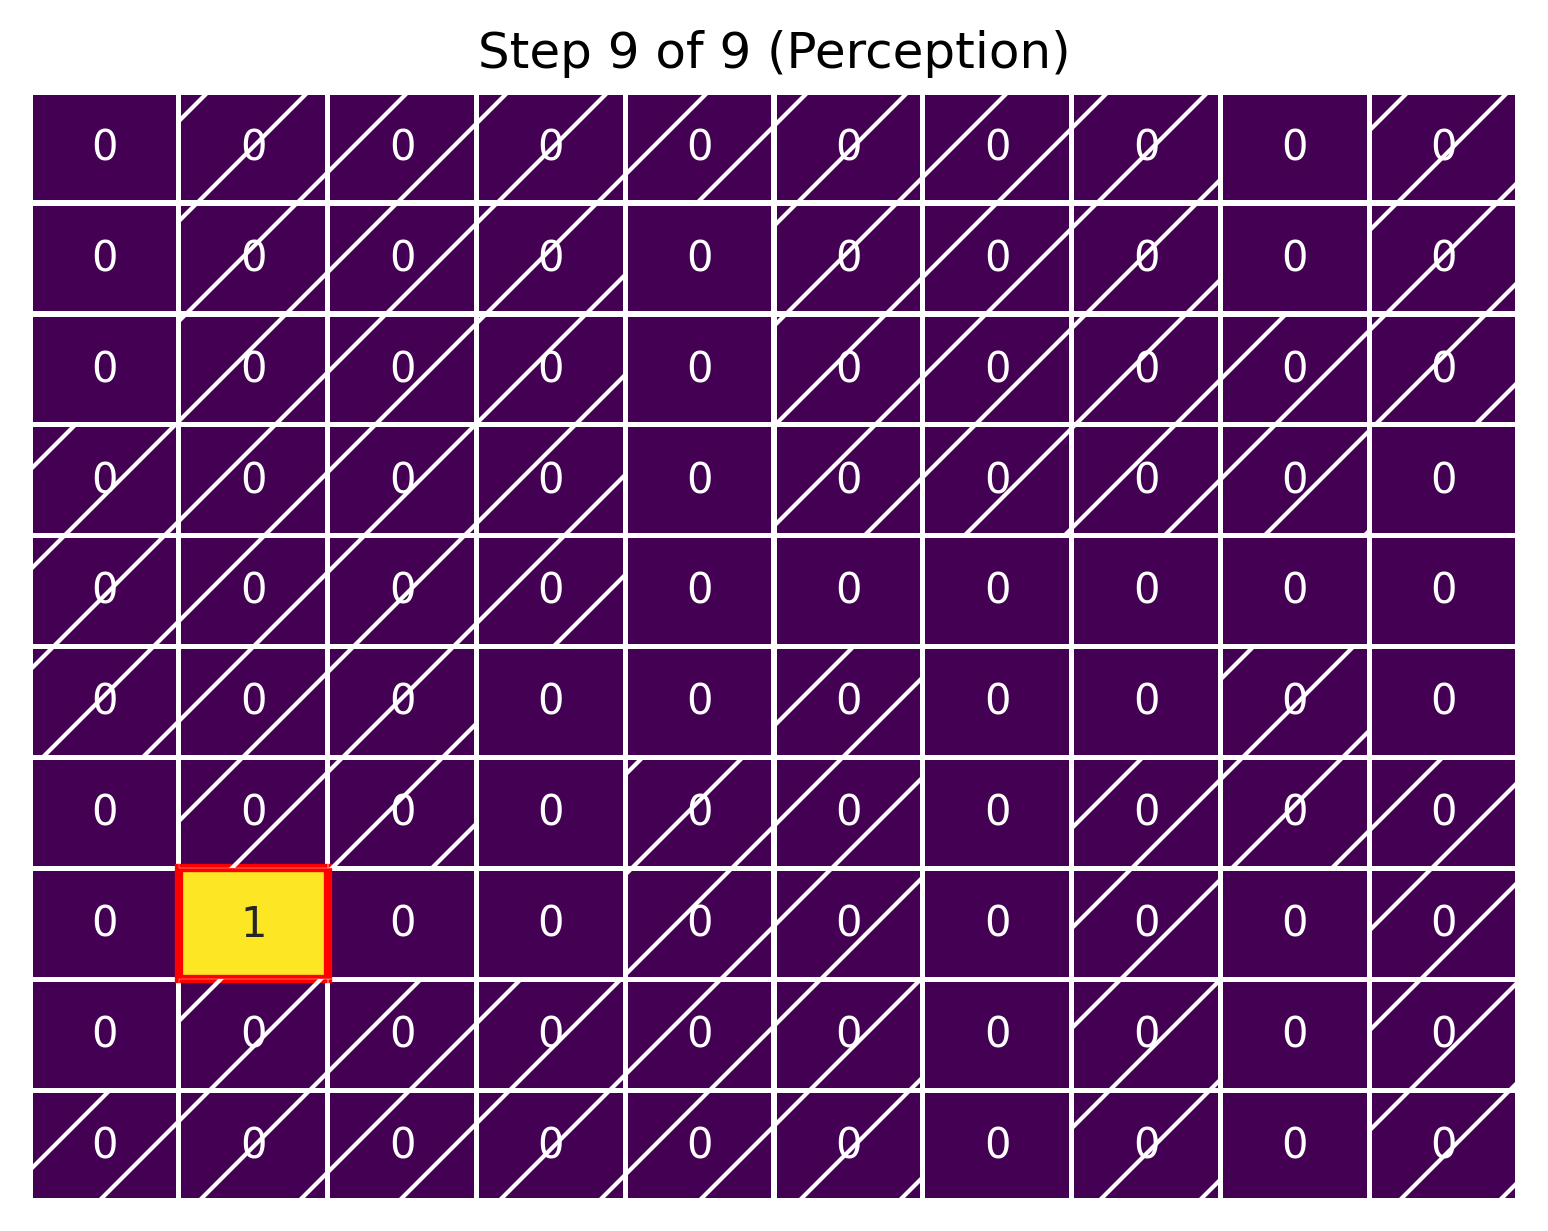
\includegraphics[width = 0.3\textwidth]{maps/Step 9 of 9 (Perception).png}}
    \end{tabular}
    \caption{A sampled execution of the markov localization algorithm. The box with the red outline is the actual location of the robot, unknown to the localization algorithm. The hatched out cells are walls. Numbers on the boxes represent beliefs for each location.}
    \label{fig:2}
\end{figure}

\newpage

\section{Mapping}

This part of the project is implemented in ROS.
The robot platform chosen is TurtleBot3.
The robot is moved in the environment using teleoperation and a map is built from the data obtained through the LIDAR sensors on the robot.
This data is transformed from the robot's frame of reference to the word frame and is visualized in an RViz window. It is demonstrated in the following video: \href{https://youtu.be/EWWotzJBU4A}{https://youtu.be/EWWotzJBU4A}.
The pose of the robot is estimated by fusing the sensor data from the inertial measurement unit of the robot as well as it odometry sensors, these are then fed into an Extended Kalman filter to obtain the estimate of the pose.

The code for this part is also available in the github repository: \href{https://github.com/say4n/mobile-robotics}{https://github.com/say4n/mobile-robotics}.


\vspace{2cm}

\hrule

\vfill
\hrule
\hrule

%----------------------------------------------------------------------------------------

\end{document}